\documentclass[]{article}
\usepackage[utf8]{inputenc}
\usepackage{natbib}
\usepackage{graphicx}
\usepackage{geometry}
\usepackage{hyperref}

\usepackage{listings}
\usepackage{xcolor}
\usepackage{multicol}

\definecolor{codegreen}{rgb}{0,0.6,0}
\definecolor{codegray}{rgb}{0.5,0.5,0.5}
\definecolor{codepurple}{rgb}{0.58,0,0.82}
\definecolor{backcolour}{rgb}{1,1,1}

\lstdefinestyle{mystyle}{
	backgroundcolor=\color{backcolour},   
	commentstyle=\color{codegreen},
	keywordstyle=\color{blue},
	numberstyle=\tiny\color{codegray},
	stringstyle=\color{codepurple},
	basicstyle=\ttfamily\footnotesize,
	breakatwhitespace=false,         
	breaklines=true,                 
	captionpos=b,                    
	keepspaces=true,                 
	numbers=left,                    
	numbersep=5pt,                  
	showspaces=false,                
	showstringspaces=false,
	showtabs=false,                  
	tabsize=2
}

\lstset{style=mystyle}











\geometry{
	a4paper,
	total={170mm,257mm},
	left=20mm,
	top=20mm,
}

%opening
\title{Progetto di Algoritmi Avanzati  	
		\\ \large Capacitated Vehicle Routing Problem 
		 \\  Algoritmi: Costruttivi, a 2 Fasi e Genetici}
	 

\author{Giulio Pilotto - Matricola:1140718}

\date{Luglio 2019}

	

\begin{document}
	



\maketitle


\begin{abstract}

Questo elaborato presenta il progetto di Algoritmi Avanzati sottomesso al prof. Bresolin dell'Università di Padova.
Il progetto richiede di implementare almeno 2 algoritmi che risolvono istanze di : Capacitated Vehicle Routing Problem.
Nel seguente elaborato oltre ad implementare i 2 algoritmi richiesti , il primo come metodo costruttivo; Clarke and Wright e il secondo come metodo a 2 fasi:ClusterFirst - Route Second per il quale sono state implementate due tecniche di routing: Nearest-Neighbourn e Dijkastra.
Sono stati implementati altri 2 algoritmi uno che cade sempre nella classe dei metodi a 2 fasi: RouteFirst - ClusterSecond, e un altro che cade nella categoria degli algoritmi metauristici detti anche algoritmi genetici.
Inoltre, è stato implementato un metodo di selezione dei centroidi che tiene conto sia della distanza dal deposito sia della distanza inter-cluster.
Tutti gli algoritmi sono stati testati sulle 16 istanze fornite dalla libreria TSPLIB95.
I risultati confermano che a fronte di una minore accuratezza di una soluzione rispetto all'ottimo ma una maggiore richiesta di risorse in termini di tempo, possono portare a soluzioni ben approssimate.
In particolare scegliere i centrodi con il metodo RadiusRadar permette di guadagnare qualche decimo a fronte di un tempo inore.
Le soluzioni posso essere migliorate attrverso gli algoritmi genetici che fungono da esploratori di uno spazion locale.

\end{abstract}

\section{Introduzione}
Con la nascita dei nuovi servizi per il cliente, che danno assistenza e portao i prodotti direttamente sulla soglia di casa (es:Amazon Prime), la gestione della logistica predilige gran parte degli investimenti.
Questo fatto diventa ancor più importante se diamo un occhiata ai dati forniti dall' Associazione Nazionale Filiera Industria Automobilistica (ANFIA) nel 2017 \ref{fig:ITA28} , dove viene sottolineato che i camion movimentano l'80$\%$ delle merci su terra \cite{ANFIA2017}. 
Gli investimenti non riguardano solo le strutture o gli strumenti fisici, ma soprattutto i software per la gestione e l'ottimizzazione  della distribuzione dei beni.
Grazie all'informatizzazione dei processi da parte del nuovo programma di industrializzazione chiamato "industria 4.0", si può godere di banche dati ricche ed aggiornate, attraverso le quali, possono essere implementate tecniche di ricerca operativa e ottimizzazione.

Il Vehicle Routing Problem \textbf{(VRP)}  è un classe reale di problemi di soddisfacimento di vincoli, in inglese detto anche Constraint Satisfaction Problem \textbf{(COP)}.
Alla fine degli anni cinquanta Dantzig and Ramser hanno formalizzato il problema \cite{dispatching} che riguarda la distribuzione di benzina da un deposito princiapale ad un grande numero di stazioni di servizio.
Da quel momento l'interesse nei problemi VRP è evoluto da un piccolo gruppo di matematici ad un grande gruppo di ricercatori da differenti discipline ancora oggi coinvolti.


VRP consiste nell'ottimizzare l'uso di un insieme di veicoli per prelevare della merce da uno o più depositi e consegnarle presso dei clienti che richiedono una certa quantità di merce.
Le stazioni , i depositi sono distribuiti in uno spazio rappresentato da delle distanze. I mezzi si spostano percorrendo tali distanze, che possono essere rappresentate in maniera diversa.
La maggioranza the problemi reali sono sepsso più complessi del classico VRP. Quindi in pratica VRP è aumentato con dei vincoli, come ad esempio la capacità del veicolo: dove ogni veicolo è caratterizzato da una capacità limitata di carico delle merci, passando quindi da VRP a \textbf{Capacitated - VRP}.
Gli obiettivi sono molteplici:
\begin{itemize}
	\item Minimizzare dei costi di trasporto (istanze percorse, consumo di carburante)
	\item Minimizzare il numero di veicoli
	\item Rispettare il vincolo di capacità imposto  sui veicoli.
	\item Assegnare un percorso ad ogni singolo veicolo.
\end{itemize}


\begin{figure}[h!]
	\centering
	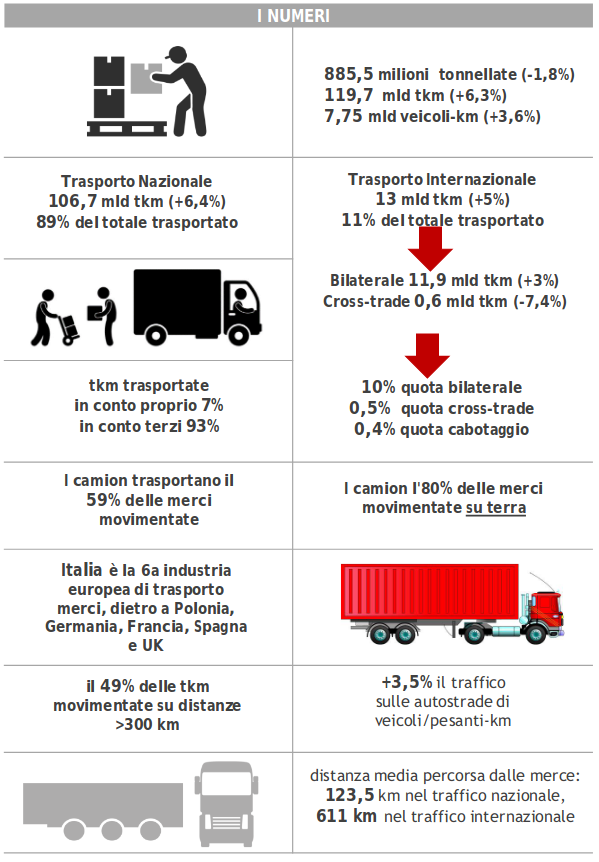
\includegraphics[scale=0.50]{images/ITA28.png}
	\caption{ Italia, traffico merci su strada, ANFIA su dati ISTAT 2017 }
	\label{fig:ITA28}
\end{figure}

VRP è un problema di ottimizzazione combinatoria NP hard,che può essere risolto esattamente trovando l'ottimo solo per piccole istanze del problema. In ogni caso gli approcci euristici che non garantiscono l'ottimalità, forniscono ottimi risultati in pratica.
Negli ultimi 30 anni sono stati applicati anche dei metodi meta-euristici che hanno mostrato una nuova direzione alla ricerca sulla famiglia di problemi VRP.
In questo elaborato vengono prese in esame le istanze fornite dalla libreria TSPLIB95\cite{TSPLIB95}.

Sono stati implementati i seguenti metodi per risolvere le istanze CVRP:
\begin{itemize}
	\item Metodo Costruttivo: Clarke and Wright
	\item Metodo a due fasi:
	\begin{itemize}
		\item Cluster-First Route-Second: Fisher and Jaikumar
		\item Route-First Cluster-Second: Dijkastra
	\end{itemize}
	\item Meta-euristiche: Algoritmi Genetici
\end{itemize}

\newpage
\subsection{Rappresentazione del problema} \label{RappProb-sec}
CVRP è la versione più comune dei problemi VRP. Ciò che caratterizza queta tipologia di problemi è il fatto che l servizio è di semplice ocnsgna senza raccolta.
Inoltre le richieste dei clienti sononote a pripri e deterministiche e devono essere soddisfatte da un solo veicolo; tuti i veicoli sono identici e basati su un singolo deposito centrale. Gli unici vincoli imposti riguardano le capacità di veicoli. L'obbiettivo è minmizzare il costo totale di servizio che può essere una funzione del numero dei route, della lunghezza complessiva o del tempo di percorrenza.
Consideraimo ora la rappresentazione su grafo di questo problema.
\begin{itemize}
\item Sia \emph{G = (V,A)} un grafo completo dove \emph{V = \{0,...,n\}} è l'insieme dei vertici e \emph{A} quello degli archi.
\item I vertici \emph{i = i,...,n} corrispondono ai clienti, mentre il vertice 0 corrisponde al deposito. 
\item Ad ogni arco \emph{(i,j) $\in$ A} è associato un costo non negativo \emph{$c_{i,j}$}, che rappresenta il costo di trasferimento dall'indice \emph{i} all'indice \emph{j}
\item In genere l'uso di loop non è consentito e ciò è imposto definendo \emph{$c_{i,j}$=+$\infty$}  \emph{ $\forall$ i $\in$ V}.Nella nostra implementazione invece abbiamo definito  \emph{$c_{i,j}$=0}  \emph{ $\forall$ i $\in$ V}.
\item Dato un insieme \emph{ S $\subseteq$ V}, \emph{d(S)} denota la richiesta complessiva dei clienti in \emph{S: d(S) = $\sum_{s \in S} d_{s} $}.
\item  Indicando con \emph{r} una \emph{route}, \emph{d(r)} denota la richiesta complessiva dei vertici da esso visitati.
\item Un insieme \emph{K} di veicoli è disponibile presso il deposito. Tali veicoli sono tutti identici di capacità \emph{C}; una semplice condizione di ammissibilità del problema richiede \emph{$ d_{i} \leq C $ $ \forall i \in V \setminus \{0\} $}.
\item Ogni veicolopuò percorrere al più un \emph{route}.
\item Si assume che \emph{$K \geq K_{min}$} dove \emph{$K_{min}$} è il minimo numero di veicoli necessari per servire tutti i clienti.
\item In questa implementazione utilizziamo il numero minimo di veicoli necessari per servire tutti i vertici in \emph{S}, pari al  \emph{lower bound}  \emph{$ K_{min} =d(S)/C $}
\end{itemize}
Gli obbiettivi ed i vincoli già citati nella sezione precedente vengono ora descritti in maniera formale, associando ai vincoli il modello matematico che li esprime.

\[M_{i,j}^k = \left\{
\begin{array}{lr}
1 :sse (i,j) \in A \wedge M_{i,j} \in  r(k) \mid k \in K \wedge r \in route\\
0 :altrimenti
\end{array}
\right.
\]

Definiamo inoltre \emph{$q_{i}$} la richiesta associata ad ogni cliente visitato da un circuito e \emph{$C_{k}$} la capacità del veicolo \emph{$k \in K$}.

La funzione obbiettivo descritta formalmente è la seguente:

\begin{equation} \label{objF}
\min \sum_{k \in K} \sum_{(i,j) \in A} c_{i,j} \cdot M_{i,j}^k 
\end{equation}



al quale sono applicati i seguenti vincoli:

\begin{equation} \label{v1}
 \sum_{k \in K} \sum_{j \in V} M_{i,j}^k = 1 \ \forall i \in V
\end{equation}

\begin{equation} \label{v2}
\sum_{i \in V} d_{i} \sum_{j \in V} M_{i,j}^k \leq C_{k} \ \forall k \in K
\end{equation}

\begin{equation} \label{v3}
\sum_{j \in V} M_{0,j}^k = 1 \ \forall k \in K
\end{equation}

\begin{equation} \label{v4}
\sum_{i \in V} M_{i,h}^k - \sum_{j \in V} M_{h,j}^k = 0 \ \forall k \in K ,\  \forall h \in V
\end{equation}

\begin{equation} \label{v5}
\sum_{i \in V} M_{i,0}^k = 1 \ \forall k \in K
\end{equation}




La funzione obbiettivo \ref{objF}, minimizzare il costo dei km totali percorsi da ogni singolo veicolo.
Il vincolo \ref{v1} impone che ogni cliente deve essere servito da un solo veicolo.
Il vincolo \ref{v2} assicura che il limite sulla capacità dei veicoli venga rispettato.
I vincoli \ref{v3}, \ref{v4} , \ref{v5} sono vincoli che impongono ad ogni veicolo di partire dal deposito il nodo 0, e collegarsi ad un nodo h, unico per ogni route,e di ritornare al deposito, indicato nella nostra implementazione sempre dal nodo 0. Questi vincoli definiscono la struttura della route.
\textbf{Questa sezione va rivista }

\section{Related Works}
Quasi tutti i metodi implementati sono euristici perchè nessuno degli algoritmi può garantire di trovare una soluzione ottima per grandi istanze, in un limite di tempo computazionale ragionevole.
Un approccio euristico non esplora l'intero spazio di ricerca, piuttosto cerca di trovare una soluzione basandosi sulle informazioni che ha sul problema.
Le euristiche che risolvono istanze CVRP sono identificati come metodi costruttivi (\textbf{costructive}) e di raggruppamento \textbf{()clustering)}.
I metodi costruttivi costruiscono una soluzione gradualmente,aggiornando continuamente l'informazione che riguarda il costo, ma potrebbe non contenere nessuna fase di miglioramento o di ottimizzazione della soluzione.
Gli algoritmi costruttivi più famosi sono: Clarke and Wright's savings algorithm \cite{CK1}, \cite{CK2} , \cite{CK3} , Matching based algorithm e Multi-route improvement heuristic \cite{CK3}.
I metodi di clustering, risolvono il problema in due fasi , ed è per questo che vengono chiamati metodi a 2 fasi.  l'approccio route-first cluster second è caratterizzato dalle due fasi seguenti:
\begin{itemize}
\item \textbf{Fase 1 - Clustering:} Un algoritmo di clustering viene utilizzato per raggruppare i clienti in cluster da dare in pasto alla seconda fase
\item \textbf{Fase 2- Routing} Nella seconda fase, per ogni cluster creato nella prima fase viene ricercata la strada più corta sfruttando tecniche di ottimizzazione.
\end{itemize}
Alcuni famosi algoritmi a due fasi sono: Petal algortihm \cite{petal}, Sweep algorithm \cite{sweep} e Fisher and Jaikumar \cite{FJ}.
Questo studio investiga e compara le performance dei metodi costruttivi e di raggruppamento per risolvere istanze di CVRP.
In particolare, nell'algoritmo di Fisher and Jaikumar, è stato implementato un algoritmo per la selezione dei centroidi chiamato Radar-Radius.Questo  massimizza la distanza tra centroidi (inter-centroid distance) e la distanza tra i centroidi e il deposito in modo da garantire la migliore copertura, a seconda della distribuzione del deposito e dei clienti.
Questo algoritmo è stato implementato scegliendo un deposito per ogni istanza in TSPLIB95,solitamente il deposito con id identificativo 1.
Sono stati usati due metodi diversi per realizzare il routing tra i clienti di uno stesso cluster: Nearest Neighbourn e Dijkastra.
I raggruppamenti formati dai metodi di clustering sono successivamente ottimizzate da metodi metaeuristici, in questa implementazione viene presentato un Algoritmo Genetico  \textbf{(GA)} \cite{GA}, il quale è un famoso approccio utilizzato per risolvere istanze Travelling Salesman Problem (TSP).
\textbf{Bensi i metodi costruttivi generano già delle soluzioni molto vicino all'ottimo, l'algoritmo Genetico è applicato anche al Savings algorithm per avere una misura di performance.}




\section{Materiali e Metodi}
Lo sviluppo di algoritmi euristici è mirato a fornire una soluzione di buona
qualità ad un problema difficile con un limitato tempo di calcolo. Nella
maggior parte dei casi infatti, non si ha il tempo neccessario per applicare
metodi esatti.
In questo senso ci vengono in aiuto gli algoritmi euristici, che im-
piegano tempi di calcolo relativamente ristretti per fornire soluzioni di
buona qualità. Laport e Semet hanno fornito una classificazione di que-
sti metodi, distinguendo tra euristici classici e metaeuristici; la differen-
za principale sta nel livello di profondità che questi metodi raggiungono
nell’esplorazione dello spazio delle soluzioni. Mentre gli euristici classici
ottengono buone soluzioni con limitati tempi di calcolo, i metaeuristici
approfondiscono la ricerca della soluzione ottima nelle zone più promet-
tenti dello spazio delle soluzioni, implementando sofisticate regole di ri-
cerca e di ricombinazione dei risultati parziali ottenuti. Questi metodi,
seppur impiegando un tempo di risoluzione maggiore, ottengono soluzio-
ni migliori rispetto ai metodi classici. Rinviamo la trattazione di questi
ultimi al capitolo successivo, focalizzando ora l’attenzione sugli euristici
classici.
\subsection{Metodi Euristici Costruttivi}
Un metodo in questa categoria costruisce le strade per i veicoli mentre cerca di minimizzare la distanza percorsa.
L'algoritmo di Savings di Clarke and Wright \cite{CK1}, trova una soluzione utilizzando un'euristica, quindi il risultato non è sempre la soluzione ottima, ma dovrebbe risultare mol+to vicina all'ottimo con un risparmio di tempo computazionale elevato rispetto ad un algoritmo brute force.


\subsubsection{Algoritmo di Savings di Clarke and Wright}
L'algoritmo si basa su una coda ordinata di risparmi, detta anche \emph{savings list}.
Ogni record della coda è ottenuto collegando due \emph{route} che non hanno nodi in comune eccetto il deposito.
Dall'unione si ottiene una singola \emph{route}, come mostrato nella figura \ref{fig:saving}, dove il nodo 0 rappresenta il deposito.

\begin{figure}[h!]
	\centering
	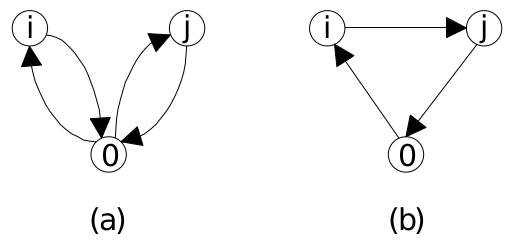
\includegraphics[scale=0.25]{images/saving.png}
	\caption{Inizialmente nella figura 1(a) i clienti \emph{i} e \emph{j} sono visitati da \emph{route} separate. Un alternativa per visitare i due clienti con la stessa \emph{route} è presentata in 1(b). }
	\label{fig:saving}
\end{figure}

I costi di trasporto calcolati in 1(a) sono:
\begin{equation}
D_{a} = C_{o,i} +C_{i,0} + C_{o,j} + C_{j,0}
\end{equation}

Mentre i costi di trasporto in 1(b) sono:

\begin{equation}
D_{a} = C_{o,i} +C_{i,j} + C_{o,j} 
\end{equation}

Ora il costo di trasporto risparmiato detto \emph{saving distance} per visitare \emph{i} e \emph{j} nella stessa \emph{route} invece che visitarli con due \emph{route} separate è:
\begin{equation}
D_{a} = D_{a} +D_{b} =+ C_{i,0} +  C_{0,j} +  C_{i,j} 
\end{equation}

\paragraph{Sequenziale e Parallelo } \hfill
La distanza risparmiata è direttamente proporzionale alla vicinanza dei clienti e inversamente proporzionale alla vicinanza al deposito.
Più grande è la distanza risparmiata più vicini si troveranno i clienti, e più distanti essi saranno dal deposito.
Le coppie di clienti sono ordiate in ordine decrescente secondo il valore di \emph{savings} che è stato calcolato sulla coppia.
La costruzione delle \emph{routes} parte dal primo record della coda. Quando una coppia \emph{i}  e \emph{j} viene considerata se questa è già presente in una \emph{route} allora si passa alla prossima coppia per l'inserimento.
Ci sono due approcci proposti per l'algoritmo di \emph{savings} \textbf{sequenziale}  e \textbf{parallelo}.
\begin{itemize}
\item Nell'approccio \textbf{sequenziale} se una coppia di cliente non corrisponde con uno dei nodi presenti nella strada, la coppia viene ignorata.
Ogni volta che un cliente è inserito in una \emph{route}, l'algoritmo deve cominciare dall'inizio siccome le combinazioni che non erano disponibili fino a prima dell'inserimento potrebbero essere disponibili ora. Questo approccio crea una \emph{route} alla volta, richiedendo di ripassare la coda di \emph{savings} più di una volta.
Il codice allegato Listing1 descrive come è stato implementato l'algoritmo sequenziale di Clarke and Wright.
La riga 2 e 3, importano il valore di capacità per ogni veicolo, e la rispettiva domanda di ogni cliente. Alla riga 4, la lista di savings viene calcolata attraverso la funzione \emph{calculateSavings} per ogni arco presente nel grafo. Alla riga 8 l'istruzione di controllo \emph{while}, continua a eseguire il codice al suo interno fino a quando tutti i clienti sono assegnati ad una \emph{route} e la lista di  \emph{savings} contiene elementi di risparmio. All'interno del \emph{while} alla riga 9 viene estratta la prima coppia di risparmi,alla riga 10 si inizializza il puntatore \emph{k}, che servirà a scorrere la lista \emph{savings} durate la costruzione della strada \emph{route}, inizializzata poco più sotto alla riga 12, dopo l'istruzione di controllo \emph{if} che controlla che nessun componente della coppia sia già servito da un'altra \emph{route} e che nessuna \emph{route} sia stata già creata. Se il controllo risulta vero allora si passa all'inizializzazione della strada con la coppia selezionata \emph{pair} e quindi si prosegue scorrendo il resto della lista \emph{savings} alla riga 14. Al suo interno i controlli alla riga 18 e 23, garantiscono al mutuale esclusività dei componenti della coppia all'interno della strada che viene estesa dalle rispettive istruzioni 20 e 25; in 21,22 \emph{k} viene azzerato e \emph{save} tolto dalla lista \emph{savings},per ricominciare dall'inizio della lista e scorrere eventuali coppie che adesso potrebbero essere collegate, grazie ai nuovi clienti. Le istruzioni solo uguali in 26,27. Le istruzioni di controllo 19 e 24, garantiscono che il cliente aggiunto rispetti i vincoli di capacità del veicolo, in caso questo.  Infine in 30 si aggiunge la \emph{route} alla soluzione e 31 aggiorna la lista \emph{savings} con la nuova distanza della coppia \emph{pair}. In 32 si ritorna la soluzione.

\item  L'approccio \textbf{parallelo} crea più \emph{routes} contemporaneamente.Quando una coppia di clienti è presa in considerazione, viene confrontata con tutte le \emph{routes} che sono già state generate fino a quel momento.
Se la coppia viene inserita in una route, tutte le \emph{routes} generate fino ad ora vengono confrontate per trovare possibili \emph{route} da unire ulteriormente con attraverso un \emph{merge}. Altrimenti,se la coppia di clienti non corrisponde con nessuna \emph{route},allora una nuova \emph{route} viene create, questa nell'approccio sequenziale invece verrebbe scartata. Nella versione parallela la lista dei \emph{savings} viene visitata una sola volta per tutta la sua lunghezza.
Nel codice Listing2 Dalla riga 2 alla riga 6 le istruzioni sono identiche al codice Listing 1 già presentato. Dalla riga 7 invece si differenzia, in quanto per ogni cliente viene creata una strada: deposito $\rightarrow$ cliente $\rightarrow$ deposito. In 0 il ciclo \emph{for} si occupa di scorrere la lista. Al suo intenro a riga 10 si estrae la tupla che forma la coppia di clienti che appartengono al risparmio. 11,12 e 13 inizializzano a \emph{null} tre di appoggio contenitori \emph{route}. Una volta estratti i clienti, si scorrono tutte le \emph{routes} come in 14, il controllo in 15 si controlla se una \emph{route} passa per \emph{i}, quando questa viene trovata, viene allocata sia in \emph{routeA} in 16, la stessa cosa viene fatta per \emph{j} in 18, 19 con  \emph{routeB}. Il senso di questa doppio allocazione viene si spiega nella righe successive: in 22 si verifica se  \emph{routeA} e \emph{routeA} hanno valori diversi, siccome tutti i clienti hanno una strada assegnata, \emph{routeA} e \emph{routeB} saranno sicuramente diverse da \emph{null} di conseguenza si controlla in 21 se \emph{i} e \emph{j} provengono da strade diverse. In caso positivo si controlla se i componenti della \emph{routeA} e i componenti della \emph{routeB}  rispettano i vincoli di capacità, come descritto in riga 22.Se anche questo controllo viene passato con successo, allora si passa al metodo fondamentale di questo algoritmo, \emph{il Merge}	riga 23.
Questo metodo si preoccupa di capire se i due clienti presenti nelle due diverse \emph{route}, stanno in testa o in coda alla \emph{route}, di conseguenza unisce le due strade importando i clienti nella \emph{routeA} o nella \emph{routeB} a seconda dell'ordine dato da \emph{save}. In 24 si rimuove da \emph{routes} la \emph{route} che è stata copiata e in 26 si ritorna la soluzione.
\end{itemize}
\textbf{
La differenza sostanziale tra i due metodi è la seguente: il metodo sequenziale tende a generare una \emph{route} unica molto grande, e le \emph{route} seguenti invece sono più piccole. Mentre il metodo parallelo tende a formare più strade larghe e quindi riduce il numero finale di \emph{routes}} 

\begin{lstlisting}[language=Python, caption=Implementazione sequenziale di Clarke and Wright  ,escapeinside={(*}{*)}]
def Clarke&Wright_Sequenziale(graph):
	Capacity = graph.getCapacity()
	Demands:list = graph.getDemands()
	list savings = []calculateSavings (i,j) (* $\forall \ i,j \ \in V \mid i \neq j \wedge i \neq 0 $*)]
	savings.sort(descending)
	list routes = []
	
	while((*$ \sum_{(r) \in R} \sum_{(v) \in V} ( v \in r) \neq  \ \mid V \mid $*) and len(savings)>0):
		pair = savings.popFirst()
		k=0
		if(pair not served yet and No route is selected):
			route = Route.create(pair)
			
			while(k< lenghtOf(savings)):
				save = savings[k]
				i , j = tuple(save)
				k=k+1
				
				if(route already served i):
					if(checkCustomer(j)):
						route.AddCustomer(j)
						k=0
						savings.remove(save)							
				elif (route already served j):
					if(checkCustomer(i)):
						route.AddCustomer(i)
						k=0
						savings.remove(save)				
					
			routes.append(route)
			savings.update(route)
					
	return routes	
				
\end{lstlisting}


\begin{lstlisting}[language=Python, caption=Implementazione parallela di Clarke and Wright  ,escapeinside={(*}{*)}]
def Clarke&Wright_Parallelo(graph):
	Capacity = graph.getCapacity()
	Demands:list = graph.getDemands()
	list savings = [calculateSavings (i,j) (* $\forall \ i,j \ \in V \mid i \neq j \wedge i \neq 0 $*)]
	savings.sort(descending)
	list routes = []
	routes.append([0 - i - 0])  (* $\forall \ i \ \in V \mid i \neq 0 $*) 
	
	for save in savings:
		i , j = tuple(save)
		routeA = null
		routeB = null
		routeSelected = null
		for route in routes
			if route.served(i):
				routeA = route

			elif route.served(j)
				routeB = route
					    
		if rotues.index(routeA) != routes.index(routeB):
			if routeA.capacity() + routeB.capacity() <= Capacity:
				Merge(routeA,RouteB) 
				routes.remove(RouteA or RouteB)
				
	return routes
\end{lstlisting}

\subsection{Metodi Euristici di Raggruppamento (Clustering)}
I metodi di raggruppamento chiamati anche clustering method, si differenziano dagli altri metodo perchè la risoluzione del probelma è divisi a in due fasi.
\begin{itemize}
\item \textbf{Fase A} Tutti i nodi sono divisi in gruppi (cluster) utilizzando un algoritmo di raggruppamento.
\item \textbf{Fase B} Per ogni gruppo di nodi si utilizza un algoritmo di ottimizzazione per trovare il miglior routing, per servire tutti i nodi del gruppo.
\end{itemize}
Ecco perchè questi algoritmi sono conosciuti anche come algoritmi a 2 fasi.
In questo elaborato vengo presentati i seguenti metodi di raggruppamento a due fasi:
\begin{itemize}
	\item Cluster First,Route Second: Fisher and Jaikumar.
		\begin{itemize}
			\item K centroid selector algoritms :  Random
			\item K centroid selector algoritms :  Radar Radius
			\item General Asignement Problem solver
			\item Routing algoritms: Nearest Neighborn
			\item Routing algoritms: Nearest Neighborn TrackPath		
		\end{itemize}
	\item Route First,Cluster Second: using an auxiliary graph and Dijkastra
\end{itemize}

\subsubsection{Algoritmo di Fisher and Jaikumar} \label{FJ-Sec}
L'algoritmo di \emph{Fisher and Jaikumar} si basa su un'assunzione il numero di veicoli per servire tutti i clienti è dato da input.
Inoltre questo metodo non è applicabile direttamente a VRP che hanno vincoli sulla distanze percorribile da parte del veicolo.
L'algoritmo si svolge in due fasi come abbiamo già detto sopra, in particolare.
\begin{itemize}
 \item Fase 1 - clustering
 	\begin{enumerate}
		\item Selezione dei centroidi: scegli un vertice \emph{k} $\in$ \emph{V} t.c. $\mid K \mid$ = \emph{numero veicoli}.
		\item Calcola il costo di inserimento $c_{i,k}$ del clienti \emph{i} al cluster \emph{k}: \\
		$a_{i,k} = min(c_{o,i} + c_{i,k}+ c_{k,0} + c_{0,k} + c_{k,i} + c_{i,0}) - (c_{0,k} + c_{k,0})  $ $ \forall k \in K$.
		\item Assegnamento Generale: risolvere un \emph{\textbf{G}eneralized \textbf{A}ssignement \textbf{P}roblem} con i costi $c_{i,k} $ $ \forall i \in V , \forall k \in K$, le richieste dei clienti \emph{D} e la capacità prestabilita \emph{C}.
 	\end{enumerate}
 \item Fase 2 - Routing: risolvere un TSP per ogni cluster.
 
\end{itemize}
	
\paragraph{Fase 1.1 - Selezione dei Centroidi} \hfill

In questo elaborato per quanto riguarda la Fase 1.1 sono stati implementati due metodi: La selezione casuale e la selezione utilizzando un algoritmo chiamato dall'autore Radar Radius.

\begin{itemize}
	\item Selezione casuale dei centroidi: vengono scelti casualmente un numero di centroidi uguale al numero di veicoli.
	\item Selezione con Radius Radar Frontier:
\end{itemize}  

\begin{equation}  \label{RR1}
max \sum_{i \in K} c_{i,0} \ 
\end{equation}

\begin{equation} \label{RR2}
c_{i,j} \geq argmax(c_{n,m})/2 \ \ \forall i,j \in K \wedge n,m \in V
\end{equation}


\begin{equation}\label{RR3}
 d_{k} \geq C/2 \ \forall k \in K  
\end{equation}

I centroidi vengono individuati con la lettera \emph{K},in quanto il numero di centroidi corrisponde al numero di veicoli. La funzione di obbiettivo \ref{RR1} massimizza la distanza dei centroidi dal deposito \emph{0}.
Il vincolo \ref{RR2} richiede ai centroidi selezionati, di rispettare una distanza che sia uguale o superiore alla metà della distanza massima tra centroidi e clienti, ovvero la distanza massima tra un centroide e qualsiasi altro cliente nel grafo. \ref{RR3} vincola i centroidi ad avere una richiesta che sia maggiore della metà della capacità del veicolo, in quanto i clienti più onerosi in termini di richiesta hanno una probabilità maggiore di risiedere in \emph{route} diverse.
I vicoli \ref{RR2} e \ref{RR3} durante l'esecuzione vengono rilassati ad ogni esplorazione dello spazio delle soluzioni, in modo da avere più clienti candidabili. In Table \ref{Table:1} viene rappresentata la selezione dei primi due centrodi, da parte dell'algoritmo.




\newpage


\begin{table}
		\begin{tabular}{c|c|c}
			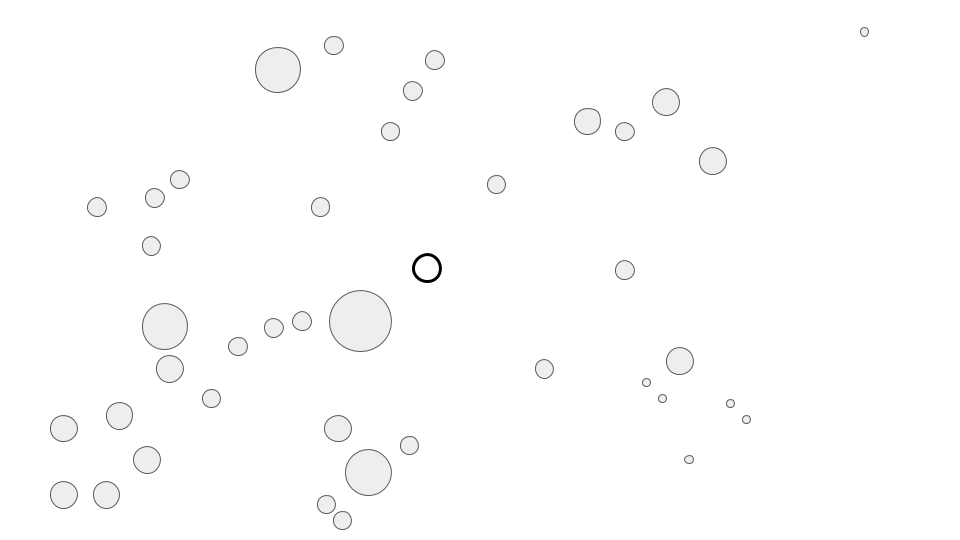
\includegraphics[scale = 0.15]{images/RR1.png} & 
			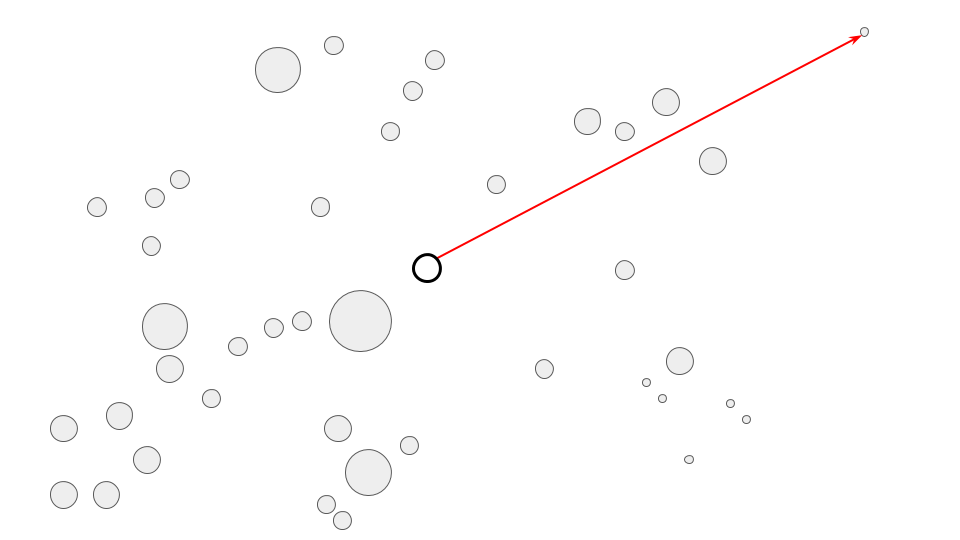
\includegraphics[scale = 0.15]{images/RR2.png}  & 
			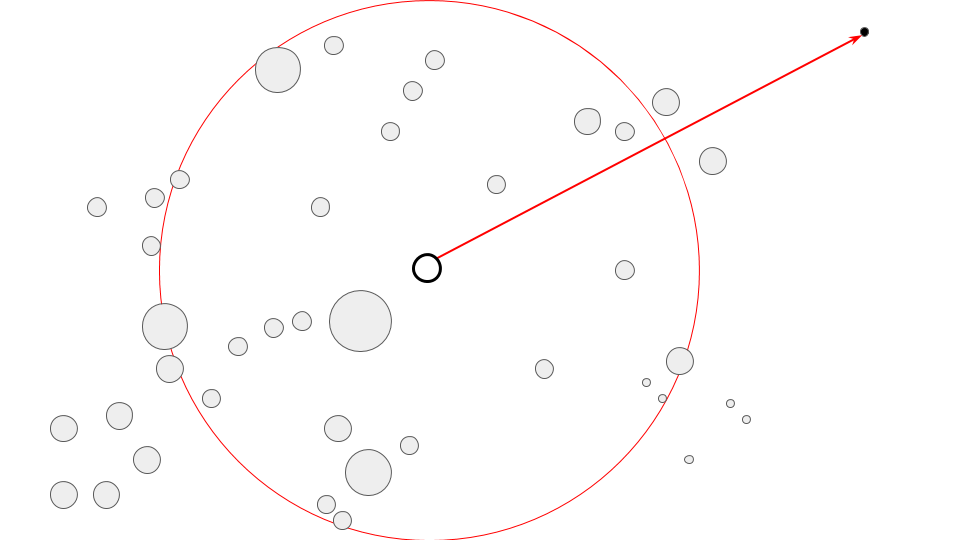
\includegraphics[scale = 0.15]{images/RR3.png}\\
			\\ \hline \\
			
			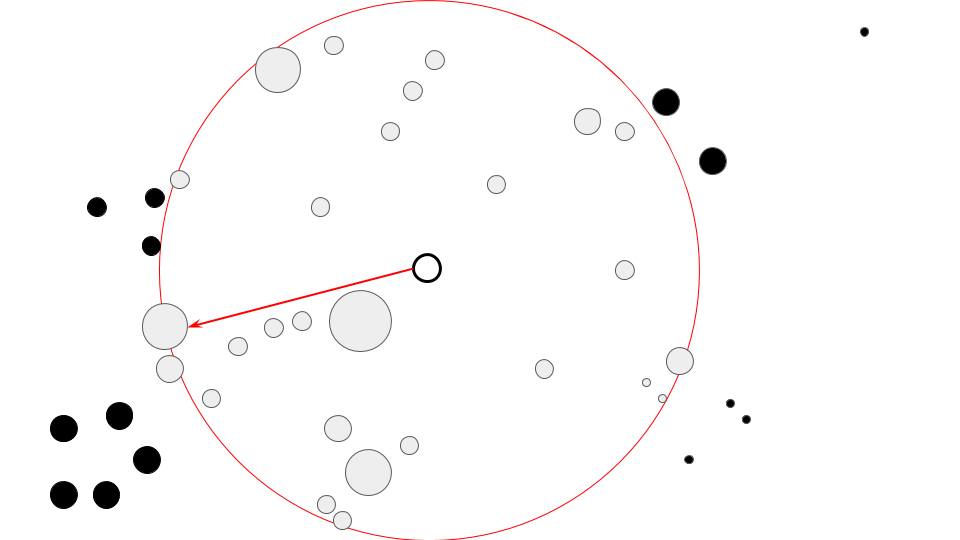
\includegraphics[scale = 0.15]{images/RR4.png} & 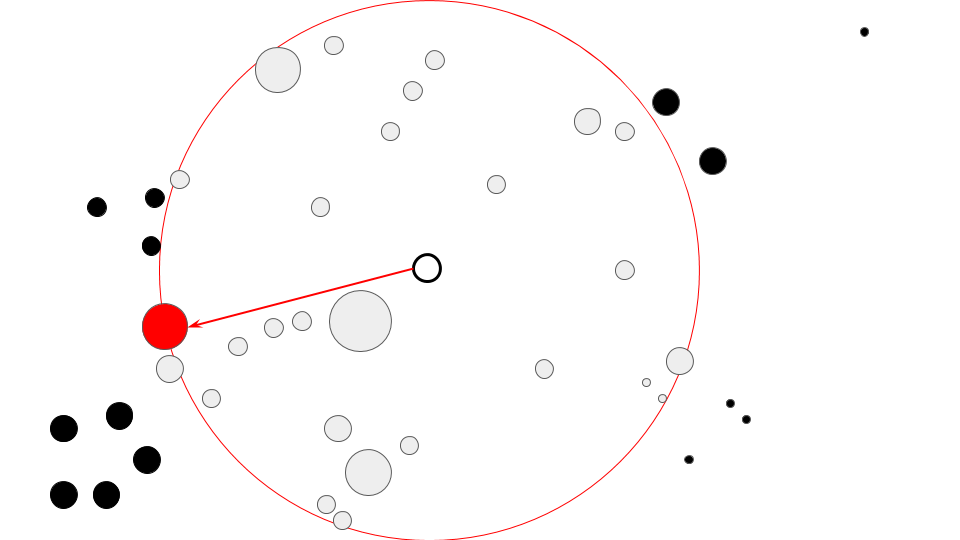
\includegraphics[scale = 0.15]{images/RR5.png} & 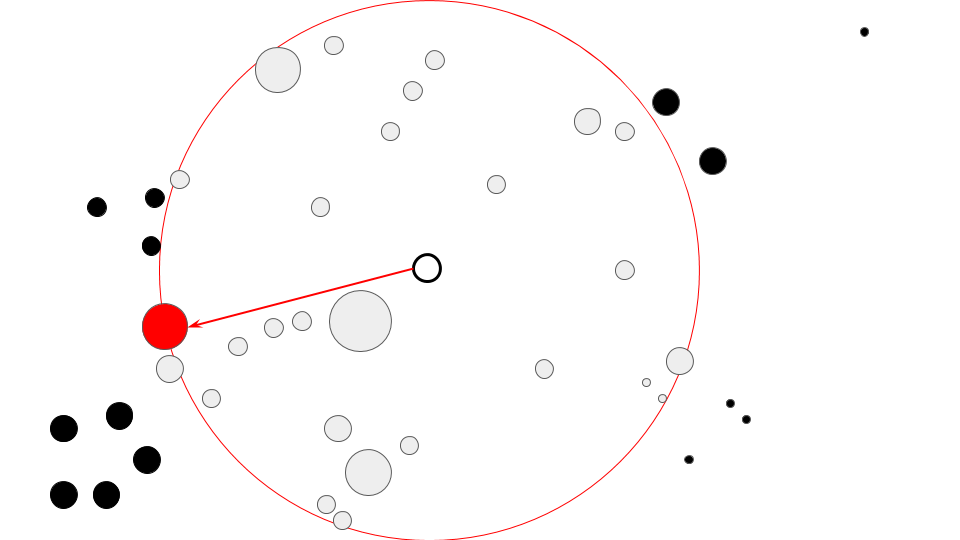
\includegraphics[scale = 0.15]{images/RR6.png}\\
			\\ \hline \\
			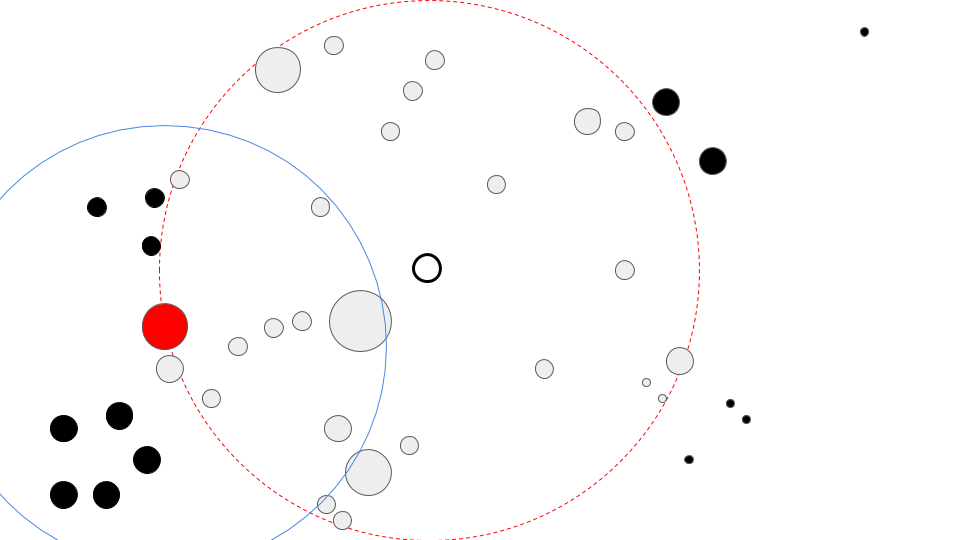
\includegraphics[scale = 0.15]{images/RR7.png} & 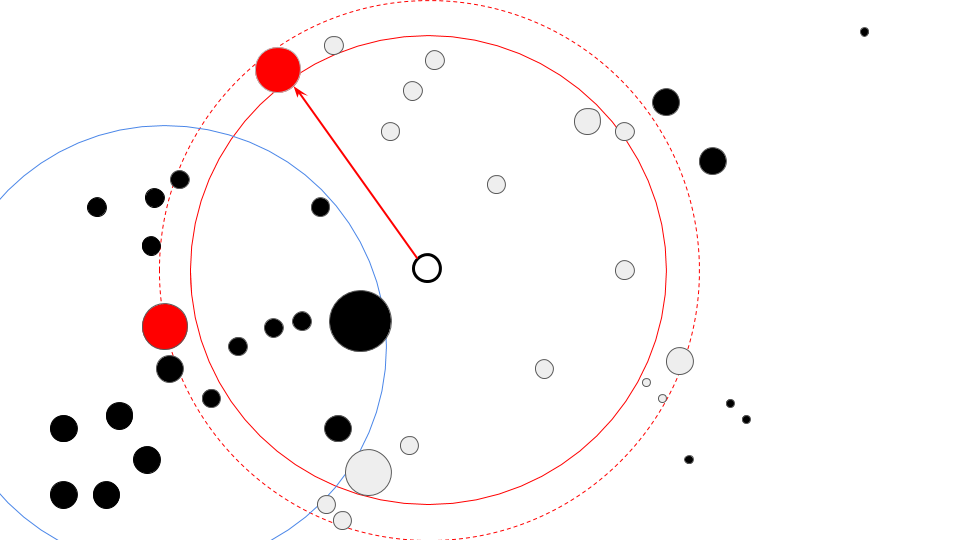
\includegraphics[scale = 0.15]{images/RR8.png} & 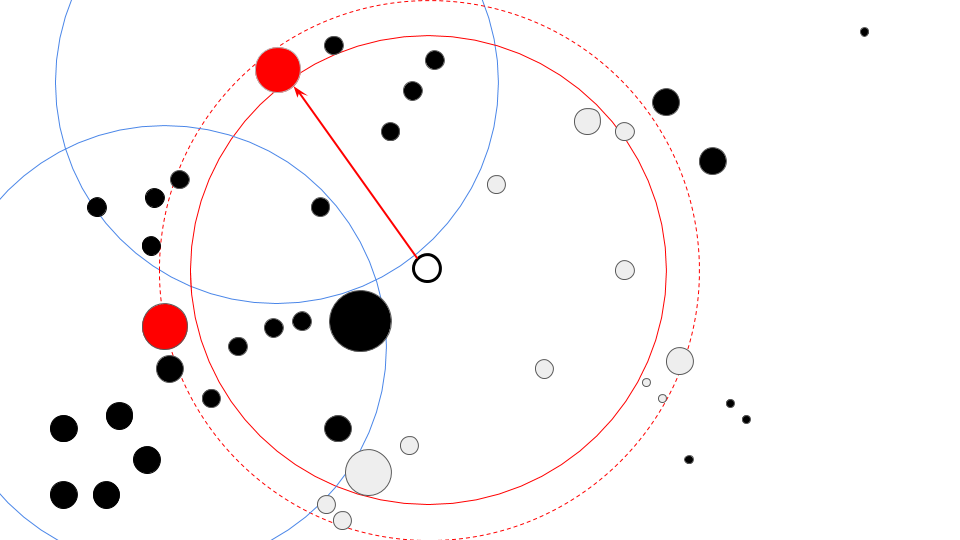
\includegraphics[scale = 0.15]{images/RR9.png}\\
						
		\end{tabular}
		\caption{In alto a sinistra il deposito al centro bianco e contorno nero, con tutti  clienti attorno da servire di colore grigio. In alto al centro l'algoritmo traccia il  raggio del utilizzando la distanza massima tra il deposito e il cliente più lontano, si definisce così il radar del deposito. Il raggio diminuisce in quanto i candidati che rispettano il vincolo \ref{RR3} si trovano più vicino al deposito,  i clienti che stazionano sulla frontiera diventano i possibili candidati, mentre gli esterni vengono esclusi,i clienti interni devono ancora essere esplorati . La figura centrale mostra il primo candidato sulla frontiera, selezionato come centroide con la distanza massima dal deposito, nella figura seguente, l'algoritmo traccia la distanza massima tra il centroide e tutti i clienti. Questa serve per tracciare il raggio del radar del centroide selezionato. Il raggio è scalato dividendolo per il numero di veicoli. Di conseguenza nella figura in basso a sinistra tutti i clienti all'interno del raggio del centroide sono esclusi dalla lista dei possibili candidati.Il raggio del radar del deposito diminuisce e dando la possibilità ad altri clienti di diventare condidati se e solo se rispettano \ref{RR3}. Viene quindi selezionato il nuovo centroide sulla frontiera e tracciato il raggio che comporrà il suo radar, come in figura in basso a destra.}
		\label{Table:1}
\end{table}

\begin{lstlisting}[language=Python, caption=RadarRadiusFrontier selettore di centroidi per Fisher and Jaikumar ,escapeinside={(*}{*)}]
def RadarRadiusFrontier(graph,n_vehicles):
	Dimension = graph.getDimension()
	Capacity = graph.getCapacity()
	Demands:list = graph.getDemands()
	scaleDown = 2
	depotDistance:list = [(*$c_{v,0} \  \forall v \in V$*)]
	seeds = []
	scannerRadius = DepotDistance
	maxCoverDistance = 0

	while (len(seeds)< n_vehicles):
		candidates = []
		if ( (*$ \sum_{i \in V} d_{i} \ \neq Dimension-1  $*)):
			for i in range(Dimension):
				if(demand[i] (*$\geq$*) capacity/scaleDown)
					candidates.append(i)
		else:
			candidates = np.arange(Dimension)
		
		for c in candidates:
			if(depotDistance[c] (*$\geq$*) argmax(scannerRadius)):
				if(seeds is empty):
					seeds.append(c)
					scannerRadius[c] = 0
					maxCoverDistance = graph.getArgMaxNodeDistance(c)
					break
			
				for v in seeds:
			 		if((graph.getValue(c,v) >= maxCoverDistance/n_vehicles) and (c not in v)): 
			 			seeds.append(c)
			 			scannerRadius[c] = 0
			 			if(maxCoverDistance < graph.getArgMaxNodeDistance(c)):
			 				maxCoverDistance = graph.getArgMaxNodeDistance(c)
			 			break
			 		else:
			 			scaleDown = scaleDown + 0.5
			 			scannerRadius[c]=0
			 			continue
			 		
		if ( (*$ \sum_{i \in V} d_{i} \ \neq Dimension-1  $*)):
			print("Decrease Radius")
			scannerRadius[np.argmax(scannerRadius)] = 0
			
				
\end{lstlisting}
L'algoritmo descritto in Listing 3, presenta quanto già descritto formalmente sopra. Dalla riga 2 alla 4 si riportano le informazioni acquisite dal grafo, in 5 si inizializza il fattore di scala applicato ad ogni ciclo, che verrà aggiornato rilassando così il vincolo \ref{RR3}. In 6 si estraggono le distanze di ogni cliente dal deposito,in 7 si inizializza seeds, il contenitore di centroidi. In 8 si crea una copia di \textit{DepotDistance} andando così a creare \textit{ScannerRadius} che sarà utilizzato poi per ridurre il raggio del radar del deposito. 9 \textit{MaxCoverDistance} rappresenta la distanza massima tra centroidi e clienti.
Si inizia con la riga 11 dove il while termina solo quando avrà trovato un numero di centroidi uguale al numero di veicoli. In 13 si effettua un importante controllo: alcune istanze presenti nel dataset fornito in questo elaborato hanno una richiesta uguale per tutti i clienti spesso apri a 1. Di conseguenza se la richiesta è uguale per tutti i clienti, il vincolo sulla capacità può essere evitato, immettendo tutti i clienti come a riga 18. In caso contrario si aggiungono solo quelli che soddisfano il vincolo \ref{RR3} rilassato da scaleDown, righe 14,15,16. In 20 si scorrono tutta la lista di candidati, in 21 accetta solo i candidati con una distanza maggiore o uguale alla distanza massima tra i componenti di \textit{ScannerRadius}. Se troviamo un candidato che rispetta entrambi i controlli,in caso seeds sia vuoto possiamo aggiungerlo direttamente 22 - 26, azzeriamo il suo valore in \textit{ScannerRadius} e aggiorniamo \textit{MaxCoverDistance} con la distanza massima tra il candidato selezionato e il cliente più distante. Altrimenti scorriamo la lista di seeds, se il candidato è distante almeno \textit{MaxCoverDistance} diviso il numero di veicoli e il candidato non è già presente in seeds, lo aggiungiamo a seeds e aggiorniamo di conseguenza \textit{MaxCoverDistance}  righe 28 - -34.In caso contrario aumentiamo il fattore scaleDown e azzeriamo il candidato in \textit{ScannerRadius}. Le righe 40,41,42, vengono eseguire nel caso le richieste dei clienti siano diverse, rilassa il vincolo \ref{RR2} aumentando il bacino di candidati. 


\paragraph{Fase 2.2 e 2.3  General Assignement Problem} \hfill
Una volta individuati i centroidi si passa alla Fase 2.2. L'algoritmo deve assegnare ongni cliente ad ogni centroide. Per fare questo l'algoritmo risolve un problema di asseganemtno generale.Si richiede di trovare un assegnamento dei clienti ai cluster tale da non superare la capacità del veicolo assegnato al cluster. Il numero di chilometri totali percorsi dalla soluzione va minimizzato. Più formalmente:
\[x_{i,k} = \left\{
\begin{array}{lr}
1 :se i \ assegnato \ al \ cluster \ k \\
0 :altrimenti
\end{array}
\right.
\]

\begin{equation} \label{GAP1}
min \sum_{i \in V} \sum_{k \in K} x_{i,k} \cdot a_{i,k} 
\end{equation}

\begin{equation} \label{GAP2}
 \sum_{k \in K} x_{i,k} = 1 \ \forall i
\end{equation}

\begin{equation} \label{GAP3}
\sum_{i \in V} d_{i}  \cdot x_{i,k} \leq C \ \forall k
\end{equation}

\begin{equation} \label{GAP3}
x_{i,k} \in \{0,1\}
\end{equation}


\begin{table}
	\begin{tabular}{c|c|c}
		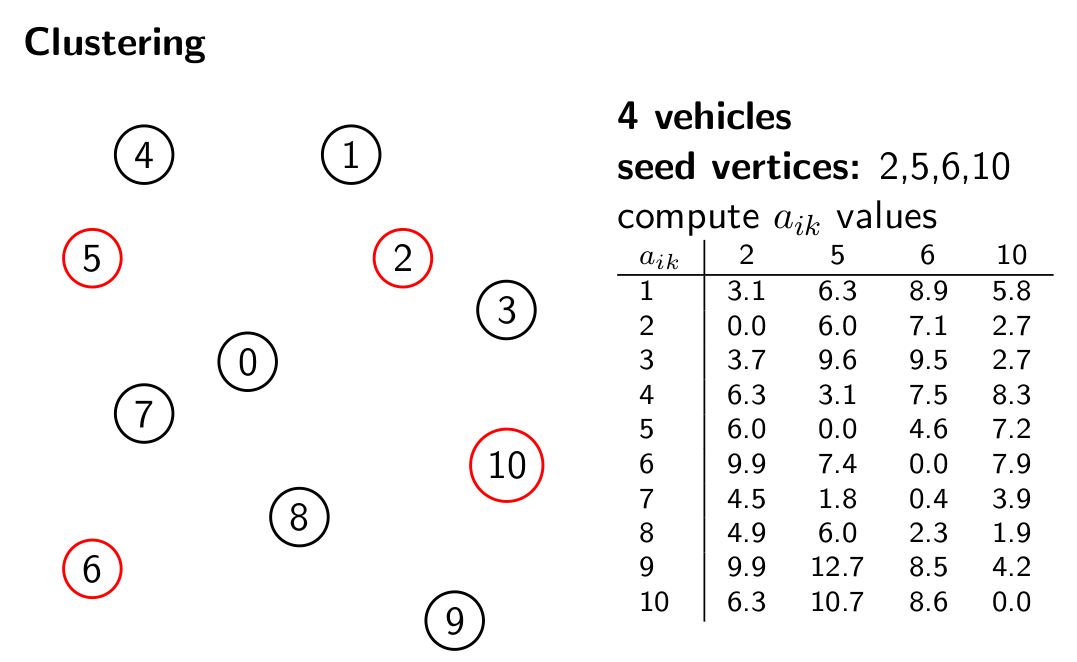
\includegraphics[scale = 0.13]{images/CL-FJ-a} & 
		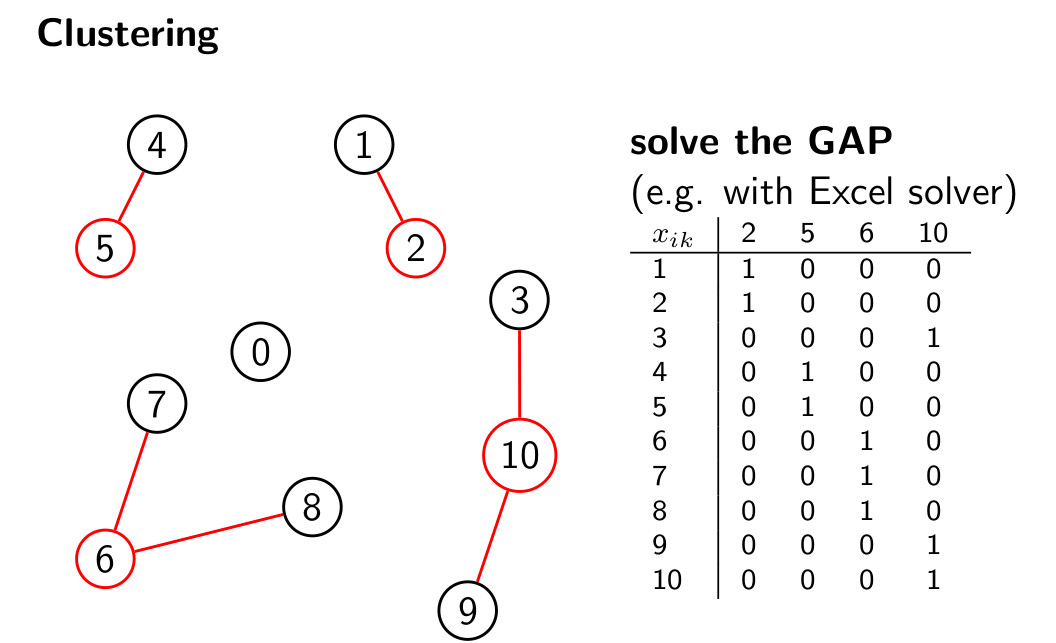
\includegraphics[scale = 0.13]{images/FJ_CL.png}  & 
		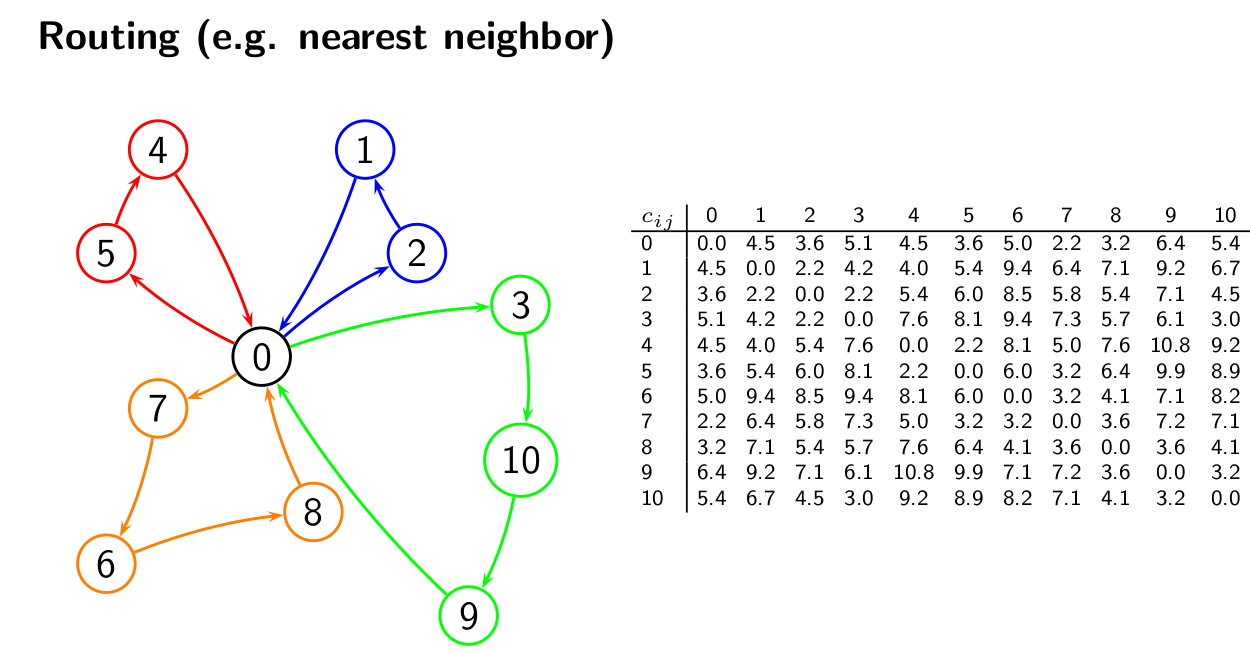
\includegraphics[scale = 0.13]{images/FJ_R.png}\\	
	\end{tabular}
	\caption{Un esempio di risoluzione GAP una volta scelto i centroidi. A sinistra vengono calcolati i costi di inserimento per ogni vertice in ogni cluster. In centro avviene l'assegnamento, associando ogni nodo al cluster che ha un costo di inserimento minore. A destra si prosegue con il routing di ogni cluster: in questo caso si usa l'algoritmo Nearest Neighbor partendo dal deposito e proseguendo verso il nodo più vicino appartenente al cluster, si prosegue per vicinanza collegando il resto dei nodi in ogni singolo cluster.}
	\label{Table:2}
\end{table}

\pagebreak

\begin{lstlisting}[language=Python, caption=General Assignement Problem solver ,escapeinside={(*}{*)}]
def GAPsolver(graph,Kclusters):
	Dimension = graph.getDimension()
	Capacity = graph.getCapacity()
	Demands:list = graph.getDemands()
	Nclusters = len(Kclusters)
	allocCosts:[list,list] = [(*$ allocCosts_{i,k} = 0 \ \forall i \in V \wedge k \in Nclusters $*)]
	clusterAssignement:list = []
	clusterDemand:list =  [(*$ clusterDemand_{k} = 0 \ k \in Kclusters $*)]
	
	allocCosts:list = [(*$ allocCosts_{i,k} =calculateIns(i,k) \ \forall i \in V \wedge k \in Nclusters $*)]
	
	i=1
	for alloc in allocCosts:
		for k in Kclusters:
			if(clusterDemand[argmin(alloc)] + Demands[i] <= Capacity):
				clusterDemand[argmin(alloc)] =+ Demands[i]
				clusterAssignment.append(np.argmin(alloc))
				i++
				break
			else:
				alloc[argmin(alloc)] = np.inf
				print("Cluster Overloaded")

	if(len(clusterAssignment)<Dimension-1):
		print("Solution is Invalid")
		return -1
	else:
		return clusterAssignment
															
\end{lstlisting}

Listing 4 presenta lo pseudocodice implementato del GAP solver implementato. Alla riga 1 la firma del metodo riceve il graph e i centroidi selezionati con le tecniche descritte nella sezione precedente.Dalla riga 2 alla riga 4 si recuperano le informazioni sul grafo, in 5 si estrae il numero di cluster. \textit{allocCosts} è la lista che conterrà i costi di allocazione di ogni cliente per ogni cluster, alla riga 5 viene inizializzata a 0 e ha dimensione uguale a \textit{Dimension}* \textit{Ncluster}. In 7 viene inizializzata a vuoto la lista \textit{clusterAssignement} che conterrà i nodi assegnati ad ogni cluster. In 8 si inizializzano a 0,il totale di domande soddisfatte per ogni cluster. In 10 vengono calcolati i costi di inserimento di ogni nodo per ogni cluster: \textit{calculateIns(i,k)} calcola i costi come è stato già descritto nella sezione \textbf{\ref{FJ-Sec}}. In 12 si inizializza il puntatore \emph{i} che servirà per puntare alla domanda del nodo corrispondente in \textit{Demands}. 13 e 14 si occupano di scorrere ogni riga di \textit{allocCosts} e al suo interno ogni cluster di \textit{Kcluster}. Il controllo a riga 15, assicura che il cluster con costo di inserimento minimo per il nodo, non superi la capacità prestabilita. Se il controllo viene superato con successo alla riga 16 si aggiorna la domanda totale soddisfatta dal cluster, in 17 si assegan al nodo il cluster e in 18 si incrementa di uno il puntatore. Siccome il nodo è stato assegnato con 19 si passa alla prossima riga di \textit{allocCosts}. Altrimenti, se il controllo a riga 15 fallisce, la riga 21 pone ad infinito il valore minimo calcolato per quel nodo, in modo che nel ciclo seguente si prenda in considerazione il secondo valore minimo calcolato tra quel nodo e un altro cluster, questo viene ripetuto per k in Kclusters.
Se alla fine dei due cicli, la lunghezza della lista \textit{clusterAssignement} non è pari al numero di nodi escluso il deposito, vuol dire che l'allocazione clienti-clusters non è andata a buon fine. Quindi la soluzione è invalida, sarà necessario aumentare il numero di veicoli e quindi si ritorna -1 . Altrimenti se tutto va bene, si ritorna l'assegnamento attraverso la lista \textit{clusterAssignement}. 

\paragraph{Fase 2 - Routing } \hfill

Ora che gli assegnamenti sono stati decisi, ci dobbiamo preoccupare di collegare i nodi all'interno di ogni cluster, in modo da formare le \emph{routes} necessarie per descrivere la soluzione. La descrizione formale di questo problema è simile a quella già descritta nella sezione  \ref{RappProb-sec}: La funzione obiettivo che descrive questa fase è la seguente:
\begin{equation} \label{objF2}
\min \sum_{k \in K} \sum_{(i,j) \in A} c_{i,j} \cdot M_{i,j}^k 
\end{equation}

\begin{equation} \label{}
M_{i,j}^k \in \{0,1\}
\end{equation}

A differenza di ciò che è descritto nella sezione  \ref{RappProb-sec} i vincoli sono già stati rispettati dalla lista di assegnamento fornita dal GAP solver.



In questa elaborato sono state utilizzate due tecniche per implementare il routing:
\begin{itemize}
\item \textbf{Nearest Neighbourn}: Partendo dal deposito ci si collega al nodo successivo, si prosegue fino a quando tutti i nodi sono stati collegati.

\begin{lstlisting}[language=Python, caption=NearestNeighbourn Routing ,escapeinside={(*}{*)}]
def Routing_NearestNeighbourn(graph,clusterAssignement,Kclusters):
	Demands = graph.getDemands()
	Capacity = graph.getCapacity()
	routes:list = []
	
	for k in Kclusters:
		cluster:list =  []
		for i in range(len(clusterAssignment)):
			if(clusterAssignment[i] == k ):
			cluster.append(i+1)
				
		appoRoute =  Route(Capacity) 
		appoRoute.addCustomer(deposit)
			
	    while(len(cluster)>0):
				prevnode = appoRoute.getLastCustmerServed()
				distPrevNode = [(*$c_{prevnode,i}  \forall i \in cluster $*)]
				nearestN = cluster[np.argmin(distPrevNode)] 
				if nearestN not in appoRoute.getCustomers():
					appoRoute.addCustomer(nearestN)
					cluster.remove(nearestN)
			
		appoRoute.addCustomer(deposit)
		routes.append(appoRoute)
			
	return routes

\end{lstlisting}
Listing 5 presenta lo pseudocodice: la firma del metodo in linea 1 richiede il grafo, l'assegnamento creato dal GAP solver, i \textit{Kcluster} selezionati dalla procedura precedente. La riga 2,3 estraggono le informazioni dal grafo, la 4 inizializza la soluzione da ritornare \textit{routes} a vuoto. Da 6 a 10 si creano i singoli cluster, scorrendo la lista \textit{clusterAssignement} e individuando a quale cluster sono stati assegnati i clienti. Per ogni cluster è creata una lista \textit{cluster}. Dentro al ciclo che scorre i cluster in 6, si inizializza la \emph{appoRoute},con capacità e deposito 12,13. Questa \emph{route} collegherà i clienti della lista  \textit{cluster} che abbiamo appena popolato. All'interno del while a riga 15, si estrae l'ultimo nodo inserito in \emph{appoRoute} e si calcolano tutte le distanze dei clienti che popolano la lista \textit{cluster} 16, 17. Si trova il più vicino al nodo estratto \textit{prevNode} 18. Se il nodo non è ancora presente nella  lista di clienti di \emph{appoRoute}, lo aggiungo e lo rimuvo dalla lista \textit{cluster} 20,21. Una volta raggiunti tutti i clienti chiudo la strada aggiungendo il deposito alal fine della lista di clienti,e aggiungo \textit{appoRoute} a \textit{routes}. Dopo aver esaurito i componenti di \textit{Kcluster}, ritorno la soluzione \textit{routes}.
\item \textbf{Nearest Neighbourn TrackPath}: Partendo dal deposito si crea una \emph{route} per ogni cliente appartenente al cluster, si espandono quindi i percorsi che hanno un costo minore. I percorsi vengono espansi aggiungendo il nodo più vicino. Infine si ritorna la \emph{route} meno costosa per ogni cluster.

\begin{lstlisting}[language=Python, caption=Nearest Neighbourn TrackPath Routing ,escapeinside={(*}{*)}]
def Routing_NN_TrackPath(graph,clusterAssignement,Kclusters):
	Demands = graph.getDemands()
	priorityQ:list =[]
	finalRoutes:list = []
	
	for k in range(len(Kclusters)):
		cluster = []
		routes =[]
		for i in range(len(clusterAssignment)):
			if(clusterAssignment[i] == k ):
			cluster.append(i+1)
	
		for node in cluster:          
			nodeRoute = Route(graph.getCapacity())
			nodeRoute.addCustomer(0)
			nodeRoute.addCustomer(node)
			nodeRoute.setCost(graph.getValue(0,node))
			priorityQ.append(nodeRoute)
		
		priorityQ.sort(key=lambda x: x.getCost(),reverse=True)
	
		while (len(priorityQ) > 0) :
			shortRoute = priorityQ.pop()
			
			prevNode = shortRoute.getLastCustmerServed()
			appoCluster:list = []
			for v in cluster:
				if v!= prevNode:
					if(v is not in shortRoute):
						appoCluster.append(v)
					
			if (len(appoCluster) > 0):
				index,value = graph.getNearestNeighbours(prevNode,appoCluster)
				costToAdd = shortRoute.getCost() + value
				shortRoute.setCost(costToAdd)
				shortRoute.addCustomer(appoCluster[index],demand[appoCluster[index]],False)
				priorityQ.append(shortRoute)
				priorityQ.sort(key=lambda x: x.getCost(),reverse=True)
				
			else:
				value = graph.getValue(prevNode,0)
				costToAdd = shortRoute.getCost() + value
				shortRoute.setCost(costToAdd)
				shortRoute.addCustomer(0,0,False)               
				routes.append(shortRoute)
			
			routes.sort(key=lambda x: x.getCost(),reverse=True)
			route = routes.pop()
			finalRoutes.append(route)
	
	return finalRoutes
\end{lstlisting}
In Listing 6 la firma del metodo è uguale a Listing 5. La  riga 2 estrae la \textit{Demand} dal grafo.
3 inizializza la priority queue \textit{priorityQ} che conterrà le strade da esplorare, ordinate in base al costo. In riga 4 si inizializza \textit{finalRoutes},la lista di \emph{routes} che sarà ritornata come soluzione. Le righe da 6 a 11 inizializzano il contenitore \textit{cluster} come già abbiamo visto nella procedura precedente. In 8 si inizializza \textit{routes} una variabile di appoggio per rendere disponibile le \emph{route} esplorate anche al di fuori del ciclo. Da 13 a 18 per ogni cliente nel cluster viene creata una \emph{route} deposito $\rightarrow$ cliente, con relativo costo, e aggiunta alla lista \textit{priorityQ}.
Al di fuori del ciclo alla riga 20 la lista viene ordinata in ordine decrescente. Si prosegue con la riga 22 dove il ciclo while controlla lo stasto della coda \textit{priorityQ}. In 23 si estrae il primo nodo della coda, che equivale alla strada più breve trovata fino a questo punto. Alla riga 22 si estrae l'ultimo nodo servito da \textit{shortRoute}. Da 26 a 30 si utilizza la lista \textit{appoCluster} per collezionare i nodi non ancora collegati a \textit{shortRoute}. In 31 si controlla la lunghezza di  \textit{shortRoute}, se contiene elementi allora si cerca il cliente più vicino a \textit{prevNode} all'interno della lista \textit{appoCluster} in riga 33. Una volta trovato il cliente, lo si aggiunge a \textit{shortRoute}, aggiornando il costo e la domanda: da riga 34 a 36. Si aggiunge la nuova \emph{route} a \textit{priorityQ}, e si ordina in ordine decrescente in 37 e 38.
Quando la lista \textit{appoCluster} non contiene più elementi si chiude la \emph{route}, aggiungendo come destinazione finale il deposito e aggiornando opportunamente i costi e la domanda: da riga 41 a 44.Infine la strada viene aggiunta a \textit{routes} 45. Quando tutte le strade sono state esploarate e collegate a tutti i nodi del cluster si sceglie la meno costosa, ordinando \textit{routes} in ordine decrescente in 47. Si  estrae la \emph{route} meno costosa in 48, e si aggiunge alla soluzione finale \textit{finalRoutes} in 49. Questa procedura viene svolta per ogni \textit{Kcluster}. Infine si ritorna la soluzione  \textit{finalRoutes}


\end{itemize}


\subsubsection{Metodo Euristico Route First, Cluster Second}
Una procedura inversa rispetto a quella che abbiamo presentato: nella prima fase si tende a costruire una grande unica \emph{route} rilassando il vicolo sulla capacità dei veicoli. Nella fase successiva si reintroduce il vincolo dividendo la singola grande \emph{route} costruita in \emph{route}  più piccole, portando il veicolo al deposito, tali da rispettare il vincolo sulla capacità. Ci sono ovviamente più modi per creare trovare una soluzione con questo metodo: si può scorrere i nodi della singola \emph{route} in ordine e ogni qualvolta la capacità eccede si chiude il tracciato e si inizia dal nodo successivo con una nuova  \emph{route}; oppure si costruisce un grafo ausiliario nel seguente modo: i nodi sono i clienti, gli archi entranti sono composti dal numero massimo di clienti che un veicolo può visitare senza superare la sua capacità compreso il nodo di partenza e di arrivo, il peso degli archi rappresenta i chilometri percorsi dal nodo di partenza al nodo di arrivo.
La rappresentazione attraverso grafo ausiliario e la conseguente applicazione dell'algoritmo di Dijkastra è l'implementazione  scelta in questo elaborato per quanto riguarda il metodo di raggruppamento route first, cluster second. In Table \ref{Table:3} un esempio esplicativo.
\begin{table}
	\begin{tabular}{c|c}
		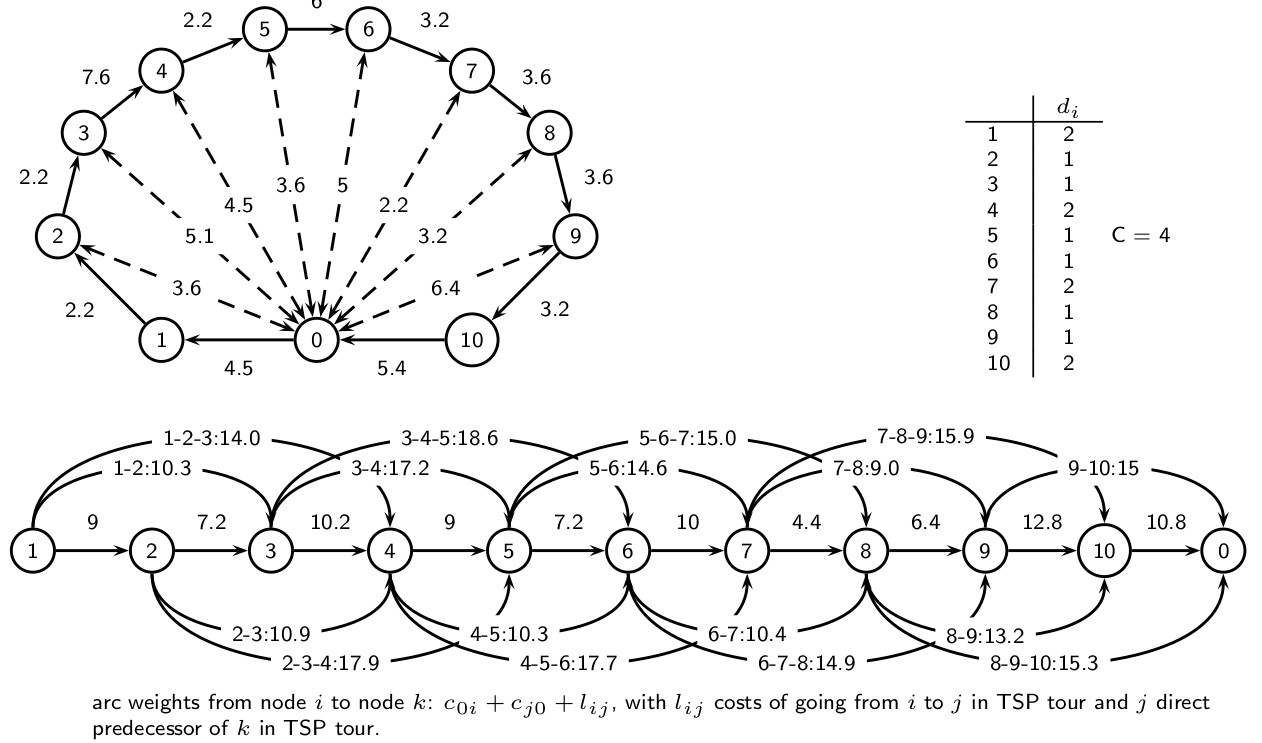
\includegraphics[scale = 0.20]{images/RFSC1.png} & 
		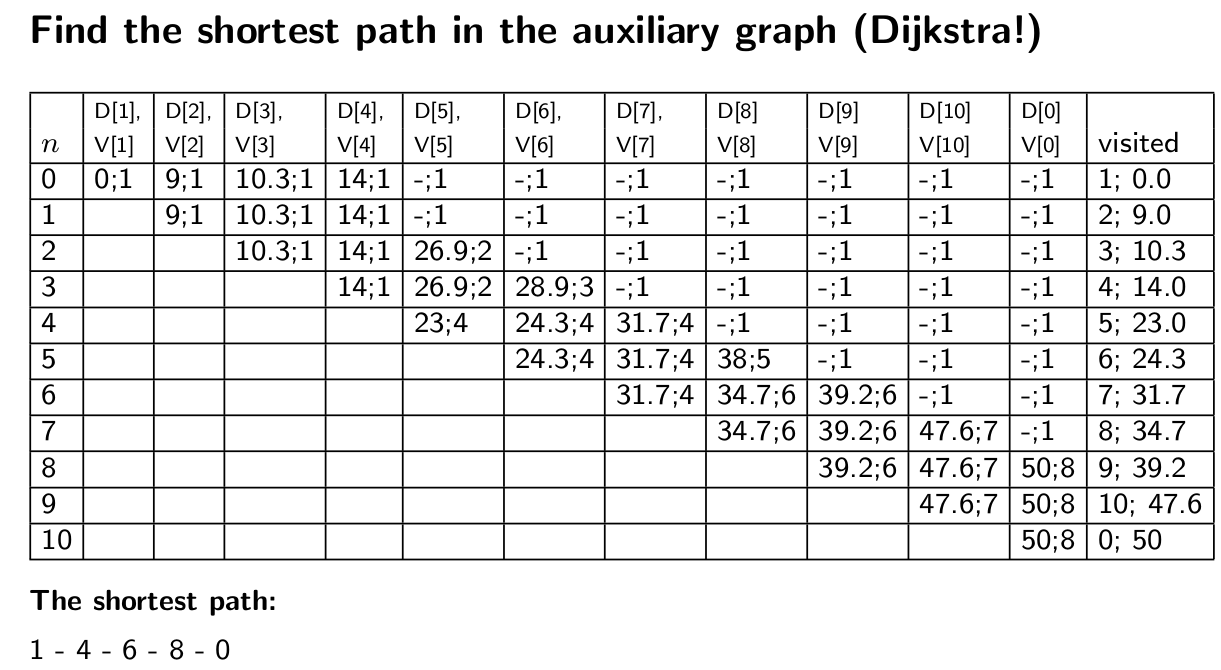
\includegraphics[scale = 0.20]{images/RFSC2.png}  
	
	\end{tabular}
	\begin{centering}
		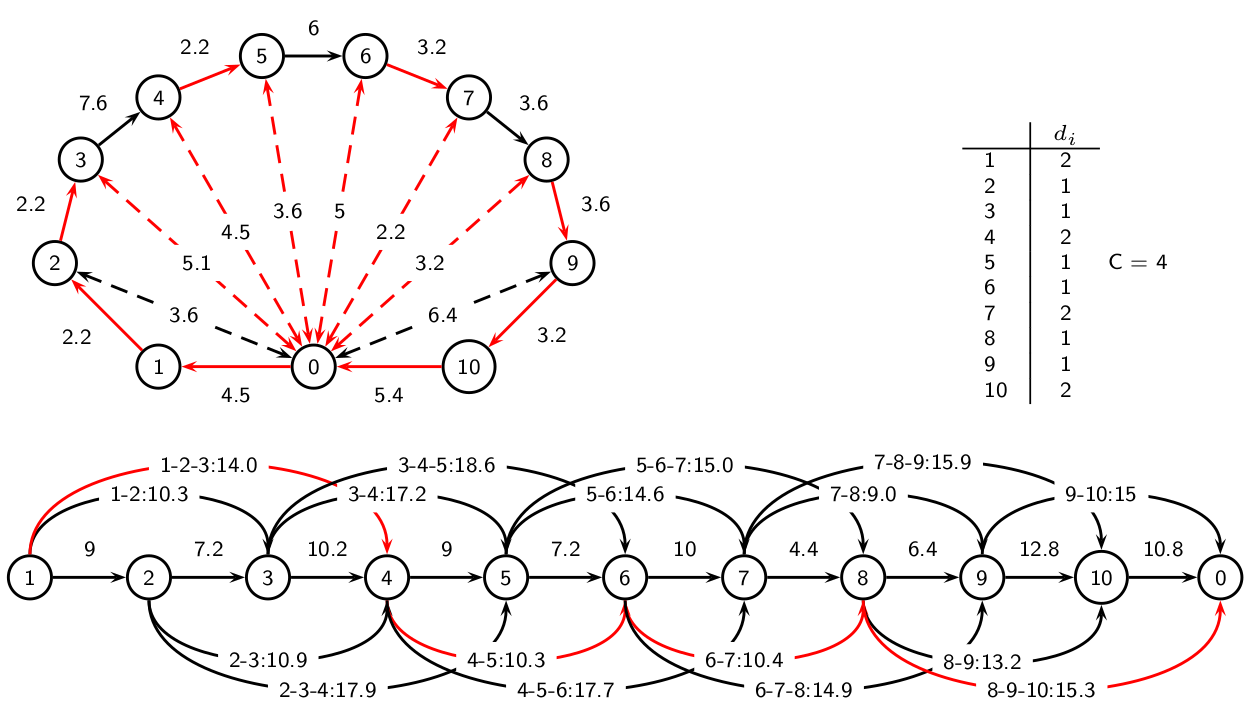
\includegraphics[scale = 0.20]{images/RFSC3.png}\\	
	\end{centering}

	\caption{Il grafo viene rappresentato escludendo il deposito,i clienti sono distirbuiti in ordine \textbf{topologico}, di conseguenza una volta arrivati al'ultimo nodo sarà sufficente procedere dall'ultimo nodo fino al primo per ricostruire la soluzione. In sostanza ogni arco del grafo rappresenta una \emph{route} l'algoritmo di Dijkastra esplora gli archi che portano al nodo finale minimizzando il costo totale del percorso,in questo caso i kilometri percorsi per ogni \emph{route}. }
	\label{Table:3}
\end{table}

\begin{lstlisting}[language=Python, caption=Route First Cluster Second con grafo ausiliario e Dijkastra  ,escapeinside={(*}{*)}]
def ClusterFirst_RouteSecond(graph):
	Capacity = graph.getCapacity()
	Demands = graph.getDemands()
	Dimension = graph.getDimension()
	dist:list = [(*$ dist_v =  \infty \ \forall v \in V $*)]
	nodeQueue:list= []
	finalRoutes:list = []
	auxGraph = [(*$auxGraph_v =(i,Route(Capacity))  \ \forall v \in V$*) ]
	
	dist[0] = 0	
	route = Route(capacity)
	route.addCustomer(0,demand[0],False)
	route.addCustomer(1,demand[1],False)
	route.addCustomer(0,demand[0],False)
 	route.setCost(graph.getValue(0,1) + graph.getValue(1,0))
	
	nodeQueue = [(1,route.getCost(),route)]
	node = 0
	nodeQueue.sort(key=lambda x: x[1],reverse=True)
	
	while (len(nodeQueue)>0):
		nodeToexpand = nodeQueue.pop()
		node = nodeToexpand[0]
		cost = nodeToexpand[1]
	
		for j in range(1,dimension):
			if(j >= node):
				newRoute = Route(capacity)
				newRoute.setCost(0)
				newRoute.addCustomer(0,demand[0],False)
				for i in range(node,j+1):
					if (i is not in newRoute and do not overload newRoute):
						newRoute.addCustomer(i)
						newRoute.setCost(newRoute.getCost()+ newRoute.getCost(lastNode,i))
					else:                            
						break
						
					newRoute.setCost(newRoute.getCost() + graph.getValue(j,0))
					newRoute.addCustomer(0)
					if(dist[j] > newRoute.getCost()+ cost):
						dist[j] = newRoute.getCost() +cost
						nodeQueue.append((j+1,dist[j],newRoute))
						auxGraph[j] = (node-1,newRoute)
						nodeQueue.sort(key=lambda x: x[1],reverse=True)
					else: break	
	
	u = len(auxGraph)-1
	while (u != 0):
		node = auxGraph[u]
		u = node[0]
		finalRoutes.append(node[1])
	
	return finalRoutes				
		
\end{lstlisting}
Listing 7 mostra alla riga 1 al firma del metodo, la quale richiede come input solo il grafo. In questo metodo non è possibile scegliere a priori il nuemro di veicoli, in quanto dipende da come viene gestito l'algoritmo di routing. Dalla riga 2 alla riga 4 si estraggono le informazioni dal grafo come abbiamo già visto precedentemente.Ala riga 5 si inizializza la lista di \textit{dist}, ovvero la lista che contiene i nodi e per ogni nodo assegna il corrispettivo numero totale di chilometri per raggiungere il nodo. In riga 6 si inizializza \textit{nodeQueue} la coda che contiene per ogni elemento, il nodo, la distanza percorsa per raggiungerlo e la \emph{route} utilizzata per raggiungere il nodo. In 7 si inizializza \textit{finalRoutes} la lista di \emph{route} che conterrà la nostra soluzione. A riga 8 viene inizializzato il grafo ausiliario \textit{auxGraph} che contiene per ogni elemento: il nodo e la strada utilizzata per raggiungerlo.
A riga 10 \texttt{dist[0]} viene assegnato a  \emph{0}, questo valore non verrà mai utlizzato durante tutta l'esecuzione dell'algoritmo, serve solamente per mantenere una coerenza con gli indici dei vertici \emph{V}. Di conseguenza dalla riga 11 alla 15 di crea la strada corrispondente al nodo sorgente, con costo uguale a 0. In 17 si inizializza \textit{nodeQueue} con il nodo sorgente, la distanza pari a alla lunghezza di  \emph{route}  e la \emph{route} corrispondente.
In 18 si inizializza la variabile \textit{node} in 19 si ordina in ordine decrescente \textit{nodeQueue}. Alla riga 21 il \texttt{while} si occupa di scorre tutta la lista \textit{nodeQueue}, fino al suo esaurimento. In 22 si estrae il nodo dalla coda \textit{nodeQueue} con costo minore, in 23 viene inserito l'indice identificativo del nodo , mentre in 24 viene riposto il suo costo. Il \texttt{for} a riga 26 crea tutti i figli del nodo, rispettando l'ordine topologico garantito dal controllo a riga 27. Per ogni figlio si crea una \emph{route} che parte dal deposito, inizializzando il costo a \emph{0}, righe da 28 a 30. Alla riga 31 il ciclo \texttt{for} scorre tutti i nodi tra il nodo estratto  \textit{node} e il figlio \emph{j+1}, 32 controlla se \emph{i} non è presente nella \textit{newRoute} e non supera il vincolo di capacità, le righe 33 e 34 lo aggiungono aggiornando il costo di \textit{newRoute} di conseguenza.
Altrimenti in si esce dal ciclo con 36, in 38 e 39 si chiude la strada. In 40 si verifica l'aggiornamento del costo dei figli esplorati confrontando il costo per arrivare la nodo figlio \textit{j} con il costo di \textit{newRoute} sommato al costo del percorso già effettuato per arrivare al nodo padre \textit{cost}. Se \textit{dist[j]} risulta maggiore, si aggiorna con il nuovo costo in 41. In 42 si aggiorna \textit{nodeQueue} con \textit{j+1} il nodo dove l'arco entra, costo dell'arco nella lista \textit{dist[j]} per arrivare al nodo  e \textit{newRoute} il collegamento tra \textit{node} e \textit{j+1}. Una volta terminato di esplorare tutti gli elementi presenti nella coda \textit{nodeQueue}, si procede estreendo l'ultimo elemento del grafo in ordine topologico e fino a quando non si arriva al nodo sorgente si risale il grafo ausiliario, percorrendo e salvando gli archi in \textit{finalRoutes}, componendo così la soluzione finale. In 53 si ritorna \textit{finalRoutes}.

\subsection{Metodi metaeuristici}
Le caratteristiche principali degli algoritmi metaeuristici sono l’esplora-
zione approfondita delle regioni, considerate più promettenti, dello spa-
zio delle soluzioni e l’impiego di sofisticate regole di ricerca del neighbo-
rhood, particolari strutture dati e metodi di ricombinazione delle solu-
zioni. Una caratteristica che spesso distingue questi algoritmi da quelli
euristici è che il procedimento di ricerca può passare attraverso soluzioni
non ammissibili e/o fasi non migliorative.
Il tempo necessario a questi algoritmi per giungere ad una soluzione
ottima è sensibilmente maggiore rispetto alle performance degli euristi-
ci classici, ma i risultati ottenuti sono solitamente di qualità superiore.
Inoltre, l’esecuzione di questi algoritmi è subordinata alla corretta valu-
tazione e impostazione di un predeterminato numero di parametri, pro-
pri dell’algoritmo stesso, al fine di adattare il metodo di risoluzione al
problema e ottenere la soluzione migliore possibile.

\subsubsection{Algoritmo Genetico}
Nel 1975 è stato proposto, da Holland, il paradigma alla base degli ago-
ritmi genetici: si tratta di una tecnica che cerca di risolvere problemi
imitando i processi tipici dell’evoluzione naturale. In via del tutto gene-
rale, l’idea di fondo consiste nel mantenere memoria di stringhe di bit,
chiamate cromosomi, rappresentanti la codifica binaria di una soluzione
al problema. L’evoluzione della popolazione è ottenuta applicando degli
operatori che simulino i più importanti fenomeni naturali: riproduzione
e mutazione.Una descrizione generica del paradigma può essere data nelle seguenti
modalità: innanzitutto sia definita una popolazione iniziale di cromosomi:
\begin{equation}
 X^1 = \{ x_{1}^1,..,x_{N}^1\}
\end{equation}
alla quale  ad ogni iterazione \emph{t = 1,..,T} sono applicate \emph{k} volte con \emph{k=N/2} le operazioni di riproduzione,ricombinazione e mutazione seguite dal passo finale di rinnovo generazionale.

\begin{itemize}
\item \textbf{Riproduzione} - Si selezionano, dalla popolazione \emph{$X^t$} , due cromosomi
generatori, privilegiando statisticamente la scelta dei cromosomi
migliori;
\item \textbf{Ricombinazione} - Si applica un operatore di crossover ai due gene-
ratori in modo da ottenere una nuova coppia di cromosomi discen-
denti ;
\item  \textbf{Mutazione} - Con piccola probabilità, si applica l’operatore di mu-
tazione ai cromosomi discendenti;
\item  \textbf{Rinnovo generazionale} - A partire da \emph{$X^t$} , si crea la popolazione \emph{$X^t+1$} rimuovendo le 2k peggiori soluzioni e sostituendole con le 2k generate nelle k precedenti applicazioni dei passi elencati.
\end{itemize}

\bibliographystyle{unsrt}
\bibliography{biblio}


\end{document}









